% This file was created by tikzplotlib v0.9.5.
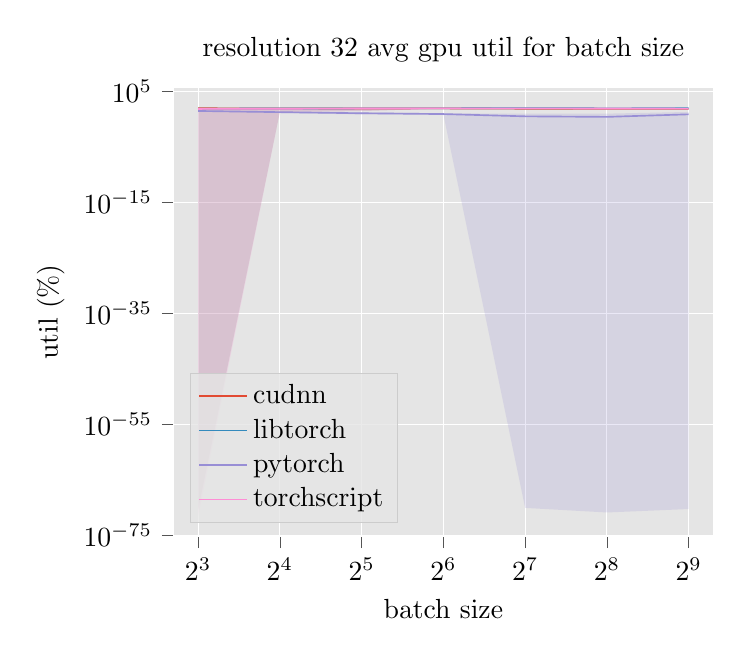
\begin{tikzpicture}

\definecolor{color0}{rgb}{0.886274509803922,0.290196078431373,0.2}
\definecolor{color1}{rgb}{0.203921568627451,0.541176470588235,0.741176470588235}
\definecolor{color2}{rgb}{0.596078431372549,0.556862745098039,0.835294117647059}
\definecolor{color3}{rgb}{0.984313725490196,0.756862745098039,0.368627450980392}
\definecolor{torchscript}{rgb}{0.996078431372549,0.556862745098039,0.835294117647059}

\begin{axis}[
axis background/.style={fill=white!89.8039215686275!black},
axis line style={white},
legend cell align={left},
legend style={fill opacity=0.8, draw opacity=1, text opacity=1, at={(0.03,0.03)}, anchor=south west, draw=white!80!black, fill=white!89.8039215686275!black},
log basis y={10},
tick align=outside,
tick pos=left,
title={resolution 32 avg gpu util for batch size},
x grid style={white},
xlabel={batch size},
xmajorgrids,
xmin=2.7, xmax=9.3,
xtick style={color=white!33.3333333333333!black},
y grid style={white},
ylabel={util (\%)},
ymajorgrids,
ymin=7.24810179764196e-76, ymax=436822.288427557,
ymode=log,
ytick style={color=white!33.3333333333333!black},
xticklabels={$2^3$, $2^4$, $2^5$, $2^6$, $2^7$, $2^8$, $2^9$},
xtick={3,...,9},
]
\path [fill=color0, fill opacity=0.2, very thin]
(axis cs:3,91)
--(axis cs:3,90)
--(axis cs:4,87)
--(axis cs:5,85)
--(axis cs:6,86)
--(axis cs:7,76)
--(axis cs:8,71)
--(axis cs:9,69)
--(axis cs:9,74)
--(axis cs:9,74)
--(axis cs:8,74)
--(axis cs:7,78)
--(axis cs:6,89)
--(axis cs:5,86)
--(axis cs:4,89)
--(axis cs:3,91)
--cycle;

\path [fill=color1, fill opacity=0.2, very thin]
(axis cs:3,82)
--(axis cs:3,74)
--(axis cs:4,80)
--(axis cs:5,85)
--(axis cs:6,85)
--(axis cs:7,91)
--(axis cs:8,89)
--(axis cs:9,89)
--(axis cs:9,93)
--(axis cs:9,93)
--(axis cs:8,91)
--(axis cs:7,93)
--(axis cs:6,91)
--(axis cs:5,91)
--(axis cs:4,85)
--(axis cs:3,82)
--cycle;

\path [fill=color2, fill opacity=0.2, very thin]
(axis cs:3,35)
--(axis cs:3,25)
--(axis cs:4,13)
--(axis cs:5,7)
--(axis cs:6,7)
--(axis cs:7,9.12835328566328e-71)
--(axis cs:8,1.36815581825213e-71)
--(axis cs:9,5.73048101459414e-71)
--(axis cs:9,20)
--(axis cs:9,20)
--(axis cs:8,10)
--(axis cs:7,10)
--(axis cs:6,11)
--(axis cs:5,19)
--(axis cs:4,22)
--(axis cs:3,35)
--cycle;

\path [fill=white!46.6666666666667!black, fill opacity=0.2, very thin]
(axis cs:3,81)
--(axis cs:3,4.38880587685435e-71)
--(axis cs:4,20)
--(axis cs:5,29)
--(axis cs:6,86)
--(axis cs:7,80)
--(axis cs:8,82)
--(axis cs:9,74)
--(axis cs:9,83)
--(axis cs:9,83)
--(axis cs:8,87)
--(axis cs:7,89)
--(axis cs:6,89)
--(axis cs:5,89)
--(axis cs:4,84)
--(axis cs:3,81)
--cycle;

\path [fill=torchscript, fill opacity=0.2, very thin]
(axis cs:3,81)
--(axis cs:3,3.40444345591596e-72)
--(axis cs:4,20)
--(axis cs:5,29)
--(axis cs:6,86)
--(axis cs:7,80)
--(axis cs:8,82)
--(axis cs:9,74)
--(axis cs:9,83)
--(axis cs:9,83)
--(axis cs:8,87)
--(axis cs:7,89)
--(axis cs:6,89)
--(axis cs:5,89)
--(axis cs:4,84)
--(axis cs:3,81)
--cycle;

\addplot [semithick, color0]
table {%
3 90.8000106811523
5 85.4999923706055
6 87.8000106811523
7 76.9999923706055
8 72.7999954223633
9 71.9999923706055
};
\addlegendentry{cudnn}
\addplot [semithick, color1]
table {%
3 79.0000076293945
4 83.5999984741211
5 87.1999969482422
7 92.0999984741211
8 89.8000106811523
9 90.9999923706055
};
\addlegendentry{libtorch}
\addplot [semithick, color2]
table {%
3 30.2500019073486
4 18.4499988555908
5 11.6499996185303
6 8.34999847412109
7 3.25000023841858
8 2.59999942779541
9 7.5
};
\addlegendentry{pytorch}
\addplot [semithick, torchscript]
table {%
3 70.2999954223633
4 76.6999893188477
5 82.6999969482422
6 88.7000045776367
8 86.4000091552734
9 80.2999954223633
};
\addlegendentry{torchscript}
\end{axis}

\end{tikzpicture}
